\documentclass{article}

\usepackage{graphicx}
\usepackage{tikz}
\usepackage{tikzsymbols}
\usetikzlibrary{calc,patterns,shapes.geometric}
\pagestyle{empty}
\usepackage[margin=0pt]{geometry}
\geometry{papersize={14in,12in}}

\def\centerarc[#1](#2)(#3:#4:#5){\draw[#1] ($(#2)+({#5*cos(#3)},{#5*sin(#3)})$) arc (#3:#4:#5);}

\begin{document}
	\begin{figure}
		\centering
		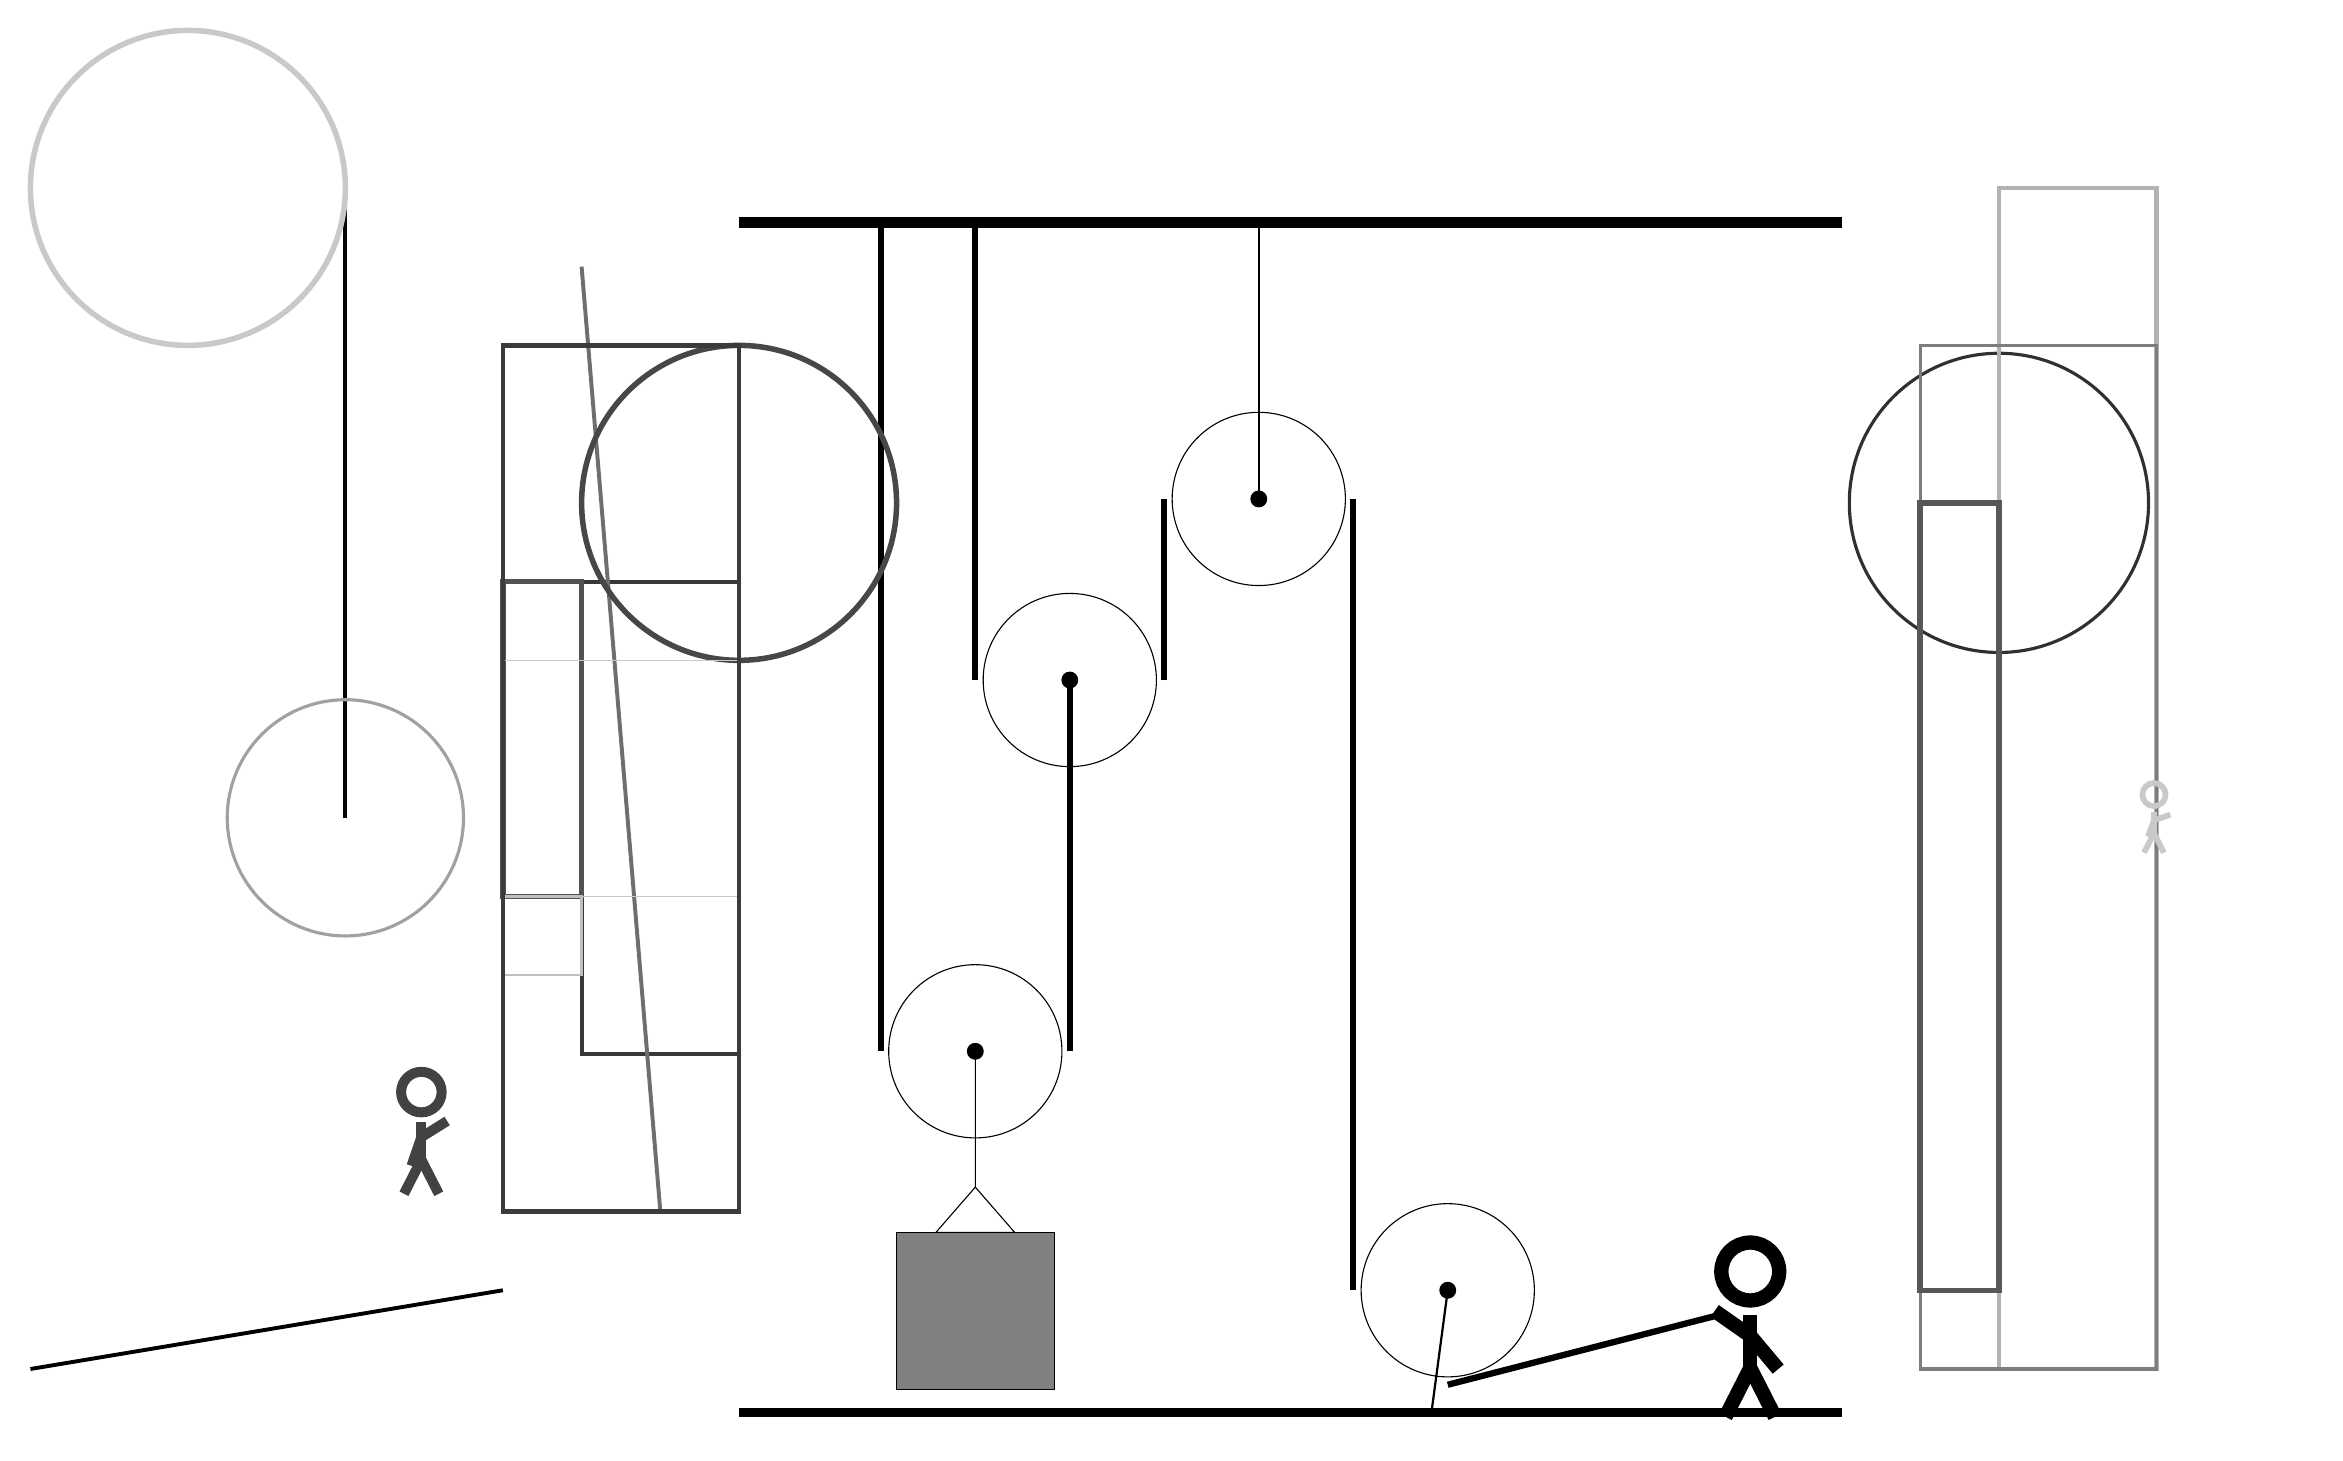
\begin{tikzpicture}
			%%%%% START %%%%%
			
			\draw[fill=black] (-2, 11.5) rectangle (12, 11.625);
			
			\draw (1, 1.035) circle (1.1);
			\draw[fill=black] (1, 1.035) circle (0.1);
			
			\draw (2.2, 5.75) circle (1.1);
			\draw[fill=black] (2.2, 5.75) circle (0.1);
			
			\draw (4.6, 8.05) circle (1.1);
			\draw[fill=black] (4.6, 8.05) circle (0.1);
			\draw[thick] (4.6, 8.05) -- (4.6, 11.5);
			
			\draw (7.0, -2) circle (1.1);
			\draw[fill=black] (7.0, -2) circle (0.1);
			\draw[thick] (7.0, -2) -- (6.8, -3.5);
			
			\draw (1, 1.035) -- (1, -0.69) -- (0.5, -1.265) -- (1.5, -1.265) -- (1, -0.69);
			\draw[fill=black!50] (0, -1.265) rectangle (2, -3.265);
			\draw[line width=0.8mm] (-0.2, 11.5) -- (-0.2, 1.035);
			\centerarc[line width=0.8mm](1, 1.035)(180:360:1.2000000000000002);
			\draw[line width=0.8mm](2.2, 1.035) -- (2.2, 5.75);
			\draw[line width=0.8mm] (1.0, 11.5) -- (1.0, 5.75);
			\centerarc[line width=0.8mm](2.2, 5.75)(180:360:1.2000000000000002);
			\draw[line width=0.8mm](3.4, 5.75) -- (3.4, 8.05);
			\centerarc[line width=0.8mm](4.6, 8.05)(0:180:1.2000000000000002);
			\draw[line width=0.8mm] (5.8, 8.05) -- (5.8, -2);
			\centerarc[line width=0.8mm](7.0, -2)(0:90:-1.2000000000000002);
			\draw[line width=0.8mm](7.0, -3.2) -- (10.5, -2.3);
			
			\node at (10.8, -2.5) {\Strichmaxerl[10][-35][-50]};
			
			\draw[line width=0.5mm, color=black!98](-7, 4) -- (-7, 12);
			
			\draw [line width=0.4mm, color=black!37](-7, 4) circle (1.5);
			\draw [line width=0.4mm, color=black!81](14, 8) circle (1.9);
			\draw [line width=0.3mm, color=black!45](18, -2) circle (0.0);
			\draw[line width=0.5mm, color=black!78] (-4, 7) rectangle (-2, 1);
			
			\draw[line width=0.6mm, color=black!30] (14, -3) rectangle (16, 12);
			
			\draw[line width=0.5mm, color=black!57](-4, 11) -- (-3, -1);
			
			\draw[line width=0.4mm, color=black!51] (13, 10) rectangle (16, -3);
			\draw [line width=0.7mm, color=black!72](-2, 8) circle (2.0);
			\draw[line width=0.7mm, color=black!68] (-4, 3) rectangle (-5, 7);
			\draw[line width=0.2mm, color=black!21] (-2, 6) rectangle (-5, 3);
			
			\draw[line width=0.5mm, color=black!100](-5, -2) -- (-11, -3);
			\node[line width=0.4mm, color=black!21] at (16, 4) {\Strichmaxerl[4][70][19]};
			
			\draw[line width=0.3mm, color=black!25] (-4, 2) rectangle (-5, 3);
			\node[line width=0.7mm, color=black!74] at (-6, 0) {\Strichmaxerl[7][71][32]};
			\draw[line width=0.7mm, color=black!66] (13, 8) rectangle (14, -2);
			
			\draw[line width=0.6mm, color=black!77] (-2, 10) rectangle (-5, -1);
			
			\draw [line width=0.7mm, color=black!21](-9, 12) circle (2.0);
			
			\draw[fill=black] (-2, -3.5) rectangle (12, -3.6);
			
			%%%%% END %%%%%
		\end{tikzpicture}
	\end{figure}	
\end{document}